%!TEX TS-program = xelatex 
%!TEX encoding = UTF-8 Unicode 
%!TEX root = ../DESpecs.tex
 

\newpage
\appendix


\section{List of All Tags}
\label{appendix list of all tags}

\newcommand{\eins}{{\fontspec{DejaVu Sans}{①}}}

\begin{longtable}[l]{@{}llll@{}l@{}}
%\begin{tabular}{@{}llll@{}}
section & tag & name & tag may contain \\[1mm]
\hline \\
\ref{section page breaks} & §<pb>§ & page break & page number & \eins \\
\ref{section page breaks} & §<rh> </rh>§ & running head && \eins \\
\\
\ref{section headings} & §<h> </h>§ & heading (or footer) && \eins \\
\ref{section paragraphs} & §<p> </p>§ & paragraph & §#§ & \eins \\
\ref{section block quotations} & §<q> </q>§ & block quotation && \eins \\
\\
\ref{section columns} & §<col> </col>§ & column & column number & \eins \\
\\
\ref{section tables basic rule} & §<tb> </tb>§ & table && \eins \\
\ref{section tables basic rule} & §#§ & \multicolumn{2}{l}{cell separator; large space} \\
\ref{section large horizontal table elements} & §\\§ & line separator && \\
\ref{section large vertical table elements} & §"§ & additional cells && \\
\\
\ref{section indexes} & §<ind> </ind>§ & index && \eins \\
\ref{section tables of contents} & §<toc> </toc>§ & table of contents && \eins \\
\\
\ref{section marginal notes} & §<mgl> </mgl>§ & marginal note (left) & anchor symbol & \eins \\
\ref{section marginal notes} & §<mgr> </mgr>§ & marginal note (right) & anchor symbol & \eins \\
\ref{section footnotes} & §<n>§ & footnote (main text) & footnote symbol \\
\ref{section footnotes} & §<fn> </fn>§ & footnote & footnote symbol & \eins \\
\ref{section anchored comments} & §<ac> </ac>§ & anchored comment & anchor symbol & \eins \\
\\
\ref{section figures} & §<fig/>§ & simple figure & \\
\ref{section figures} & §<fig> </fig>§ & complex figure & \\
\ref{section figures} & §<cap> </cap>§ & figure caption && \eins \\ 
\ref{section figures} & §<desc> </desc>§ & figure description && \eins \\ 
\ref{section figures} & §<var> </var>§ & figure variables && \eins \\ 
\\
\ref{section handwritten notes} & §<hd>§ & handwritten note & \\
\\
\ref{section characters you are unsure about} & §@§, §<gap>§ & unreadable text & \\
\ref{section characters you are unsure about} & §<?>§ & uncertain text & \\
\ref{section unknown characters} & §<001>§, etc. & unknown character & \\ 
\ref{section obvious mistakes} & §<!>§ & obvious mistake & \\
\\
\hline \\
\ref{section other diacritics} & §\'q§, etc. & character+diacritic & §' ` ^ " ~ , . = § & §-§ \\
\\
\ref{section italics} & §_ _§ & italics & \\
\ref{section bold face} & §<bf> </bf>§ & bold face & \\
\ref{section small caps} & §<sc> </sc>§ & small caps & \\
\ref{section subscript and superscript} & §<_> </_>§ & subscript & \\
\ref{section subscript and superscript} & §<^> </^>§ & superscript & \\
\ref{section underlines and overlines} & §<ul> </ul>§ & underline & \\
\ref{section underlines and overlines} & §<ol> </ol>§ & overline & \\

\ref{section text in red} & §<red> </red>§ & text in red & \\
\\
\ref{section latin ligatures} & §{quo}d§, etc. & resolved ligature & \\
%\ref{section greek ligatures} & §{μεν}§ etc. & Greek ligature & \\
\\
\hline \\
\ref{section fractions} & §{  /  }§ & fraction & \\
\ref{section roots} & §<r>§ & root & number or letter \\
\\
\hline \\
\ref{section fraktur alphabet} & §<fr>§ & \multicolumn{2}{l}{whole book in Fraktur} & \\
\ref{section fraktur alphabet} & §<fr> </fr>§ & words in Fraktur & \\
\ref{section sperrung} & §<sp> </sp>§ & Sperrung & \\
\ref{section words in roman characters} & §<rom> </rom>§ & words in roman chars & \\
\\
\hline \\
%\end{tabular}
\end{longtable}

\eins \quad This tag may also contain §it§ (italics; see \sect{section italics}) or §fr§ (Fraktur; see \sect{section fraktur}).

\newpage

\section{List of All Symbols}
\label{appendix list of all symbols}

% also: table of characters to be typed directly? MH: no
% if there is a “Symbols” section, will this appendix be unnecessary? MH: hier lassen!

\begin{tabelle}[ 1: \, common footnote symbols (from \sect{section footnotes})]
\begin{tabular}{@{}lc@{\, }c@{\, }c@{\, }c@{\, }c@{\, }c@{\, }c} \\
symbol & * & † & ‡ & \§ & ‖ & ¶ \\[2mm]
Unicode &  \xs{U+002A} & \xs{U+2020} & \xs{U+2021} &\xs{U+00A7} & \xs{U+2016} & \xs{U+00B6} \\
\end{tabular}
\end{tabelle}

\vspace{5mm}

\begin{tabelle}[ 2: \, dashes (see \sect{section dashes})]
\begin{tabular}{@{}lc@{\, }c@{\, }c@{\, }c@{\, }c@{\, }c} \\
symbol & - & – & — \\[2mm]
Unicode & \xs{U+002D} & \xs{U+2013} & \xs{U+2014} & \\
\end{tabular}
\end{tabelle}

\vspace{5mm}

\begin{tabelle}[ 3: \, common mathematical symbols (from \sect{section mathematical symbols})]
\begin{tabular}{@{}lc@{\, }c@{\, }c@{\, }c@{\, }c@{\, }c@{\, }c@{\, }c@{\, }c@{\, }c} \\
symbol & ′ & ″ & ± & \unicode{∴} & ° & ∞ & · & ÷ & √ & Ŗ \\[2mm]
Unicode & \xs{U+2032} & \xs{U+2033} & \xs{U+00B1} & \xs{U+2234} & \xs{U+00B0} & \xs{U+221E} & \xs{U+00F7} & \xs{U+00B7} & \xs{U+221A} & \xs{U+0156} \\[2mm]
\end{tabular}
\end{tabelle}

\vspace{5mm}

\begin{tabelle}[ 4: \, planet symbols (from \sect{section astronomy})]
\begin{tabular}{@{}lc@{\, }c@{\, }c@{\, }c@{\, }c@{\, }c@{\, }c@{\, }c@{\, }c@{\, }c} \\
symbol & \unicode{☿} & \unicode{♀} & \unicode{♁} & \unicode{♂} & \unicode{♃} & \unicode{♄} \\[2mm]
Unicode & \xs{U+263F} & \xs{U+2640} & \xs{U+2641} & \xs{U+2642} & \xs{U+2643} & \xs{U+2644} \\[2mm]
\end{tabular}
\end{tabelle}

\vspace{5mm}

\begin{tabelle}[ 5: \, zodiac symbols (from \sect{section astronomy})]
\begin{tabular}{@{}lc@{\, }c@{\, }c@{\, }c@{\, }c@{\, }c} \\
symbol & \unicode{♈} & \unicode{♉} & \unicode{♊} & \unicode{♋} & \unicode{♌} & \unicode{♍} \\[2mm]
Unicode & \xs{U+2648} & \xs{U+2649} & \xs{U+264A} & \xs{U+264B} & \xs{U+264C} & \xs{U+264D} \\[4mm]
symbol & \unicode{♎} & \unicode{♏} & \unicode{♐} & \unicode{♑} & \unicode{♒} & \unicode{♓} \\[2mm]
Unicode & \xs{U+264E} & \xs{U+264F} & \xs{U+2650} & \xs{U+2651} & \xs{U+2652} & \xs{U+2653} \\[2mm]
\end{tabular}
\end{tabelle}


\vspace{5mm}

\begin{tabelle}[ 6: \, technical symbols (from \sect{section technical symbols})]
\begin{tabular}{@{}lc@{\, }c@{\, }c@{\, }c@{\, }c@{\, }c@{\, }c@{\, }c@{\, }c@{\, }c} \\
symbol & \unicode{℞} \\[2mm]
Unicode & \xs{U+211E} \\[2mm]
\end{tabular}
\end{tabelle}


\newpage
\section{Example Transcriptions}

\tocspace
\subsection{Latin Example}
\label{Structural markup general example}

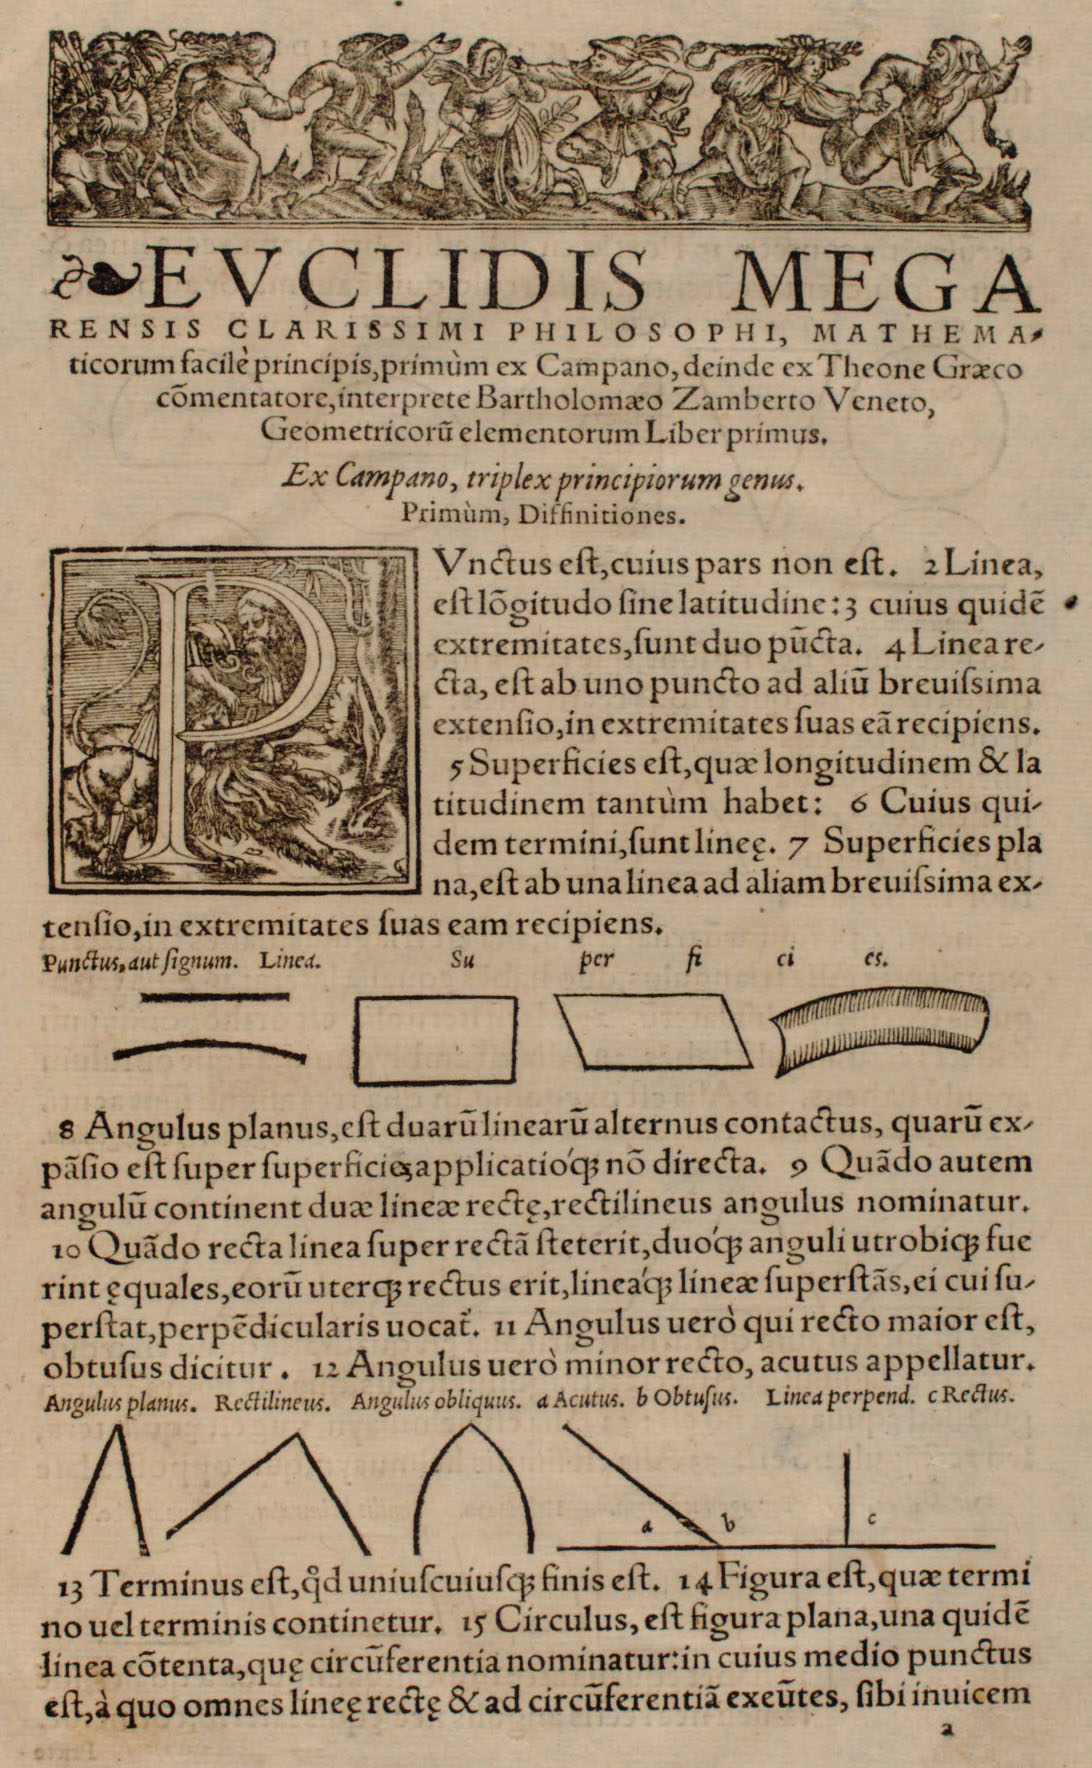
\includegraphics[height=22cm]{euclid_wholepage_3}
\clearpage

\begin{typeLatin}
\bold{<pb>} \\
\bold{<fig/>} \\
\bold{<fig/>} \\
\bold{<h>}EVCLIDIS MEGA \\
RENSIS CLARISSIMI PHILOSOPHI, MATHEMA- \\
ticorum facilè principis, primùm ex Campano, deinde ex Theone Grӕco \\
cõmentatore, interprete Bartholomӕo Zamberto Veneto, \\
Geometricorũ elementorum Liber primus.\bold{</h>} \\
\bold{<h it>}Ex Campano, triplex principiorum genus.\textbf{</h>} \\
\bold{<h>}Primùm, Diffinitiones.\bold{</h>} \\
\bold{<p>}PVnctus e$t, cuius pars non e$t. 2 Linea, \\
e$t lõgitudo $ine latitudine: 3 cuius quidẽ \\
extremitates, $unt duo p\bs\tld{}ucta. 4 Linea re-\\
cta, e$t ab uno puncto ad ali\bs\tld{}u breui$sima\\
exten$io, in extremitates $uas eã recipiens.\bold{</p>}\\
\bold{<p>}5 Superficies e$t, quæ longitudinem & la\\
titudinem tantùm habet: 6 Cuius qui-\\
dem termini, $unt line\li{ae}. 7 Superficies pla\\
na, e$t ab una linea ad aliam breui$sima ex-\\
ten$io, in extremitates $uas eam recipiens.\bold{</p>}\\
\bold{<fig>}\\
\bold{<cap it>}Punctus, aut $ignum. Linea.\bold{</cap>}\\
\bold{</fig>}\\
\bold{<fig>}\\
\bold{<cap it>}Su per fi ci es.\bold{</cap>}\\
\bold{</fig>}\\
\bold{<p>}8 Angulus planus, e$t duar\bs\tld{}u linear\bs\tld{}u alternus contactus, quar\bs\tld{}u ex-\\
pã$io e$t $uper $uperficies,\bold{<?>} applicatio´\li{que} nõ directa. 9 Quãdo autem\\
angul\bs\tld{}u continent duæ lineæ rect\li{ae}, rectilineus angulus nominatur.\bold{</p>}\\
\bold{<p>}10 Quãdo recta linea $uper rectã $teterit, duo´\li{que} anguli utrobi\li{que} fue\\
rint \li{ae}quales, eor\bs\tld{}u uter\li{que} rectus erit, linea´\li{que} lineæ $uper$tãs, ei cui $u-\\
per$tat, perp\bs\tld{}edicularis uoca\bs\tld{}t. 11 Angulus uerò qui recto maior e$t,\\
obtu$us dicitur. 12 Angulus uerò minor recto, acutus appellatur.\bold{</p>}\\
\bold{<fig>}\\
\bold{<cap it>}Angulus planus.\bold{</cap>}\\
\bold{</fig>}\\
\bold{<fig>}\\
\bold{<cap it>}Rectilineus.\bold{</cap>}\\
\bold{</fig>}\\
\bold{<fig>}\\
\bold{<cap it>}Angulus obliquus.\bold{</cap>}\\
\bold{</fig>}\\
\bold{<fig>}\\
\bold{<cap it>}Linea perpend.\bold{</cap>}\\
\bold{<desc it>}a Acutus.\bold{</desc>}\\
\bold{<desc it>}b Obtu$us.\bold{</desc>}\\
\bold{<desc it>}c Rectus.\bold{</desc>}\\
\bold{<var it>}a b c\bold{</var>}\\
\bold{</fig>}\\
\bold{<p>}13 Terminus e$t, \li{quo}d uniu$cuiu$\li{que} finis e$t. 14 Figura e$t, quæ termi\\
no uel terminis continetur. 15 Circulus, e$t figura plana, una quid\bs\tld{}e\\
linea cõtenta, qu\li{ae} circ\bs\tld{}uferentia nominatur: in cuius medio punctus\\
e$t, à quo omnes line\li{ae} rect\li{ae} & ad circ\bs\tld{}uferentiã exe\bs\tld{}utes, $ibi inuicem\\
\end{typeLatin}

\begin{note}
The typesetter used the page number of the next page as a catchword, i.e. it is not the page number of this page. The closing §</p>§ of the last paragraph is on the next page.
\end{note}

\vfill


\tocspace
\subsection{Greek Example}
\label{section greek example}

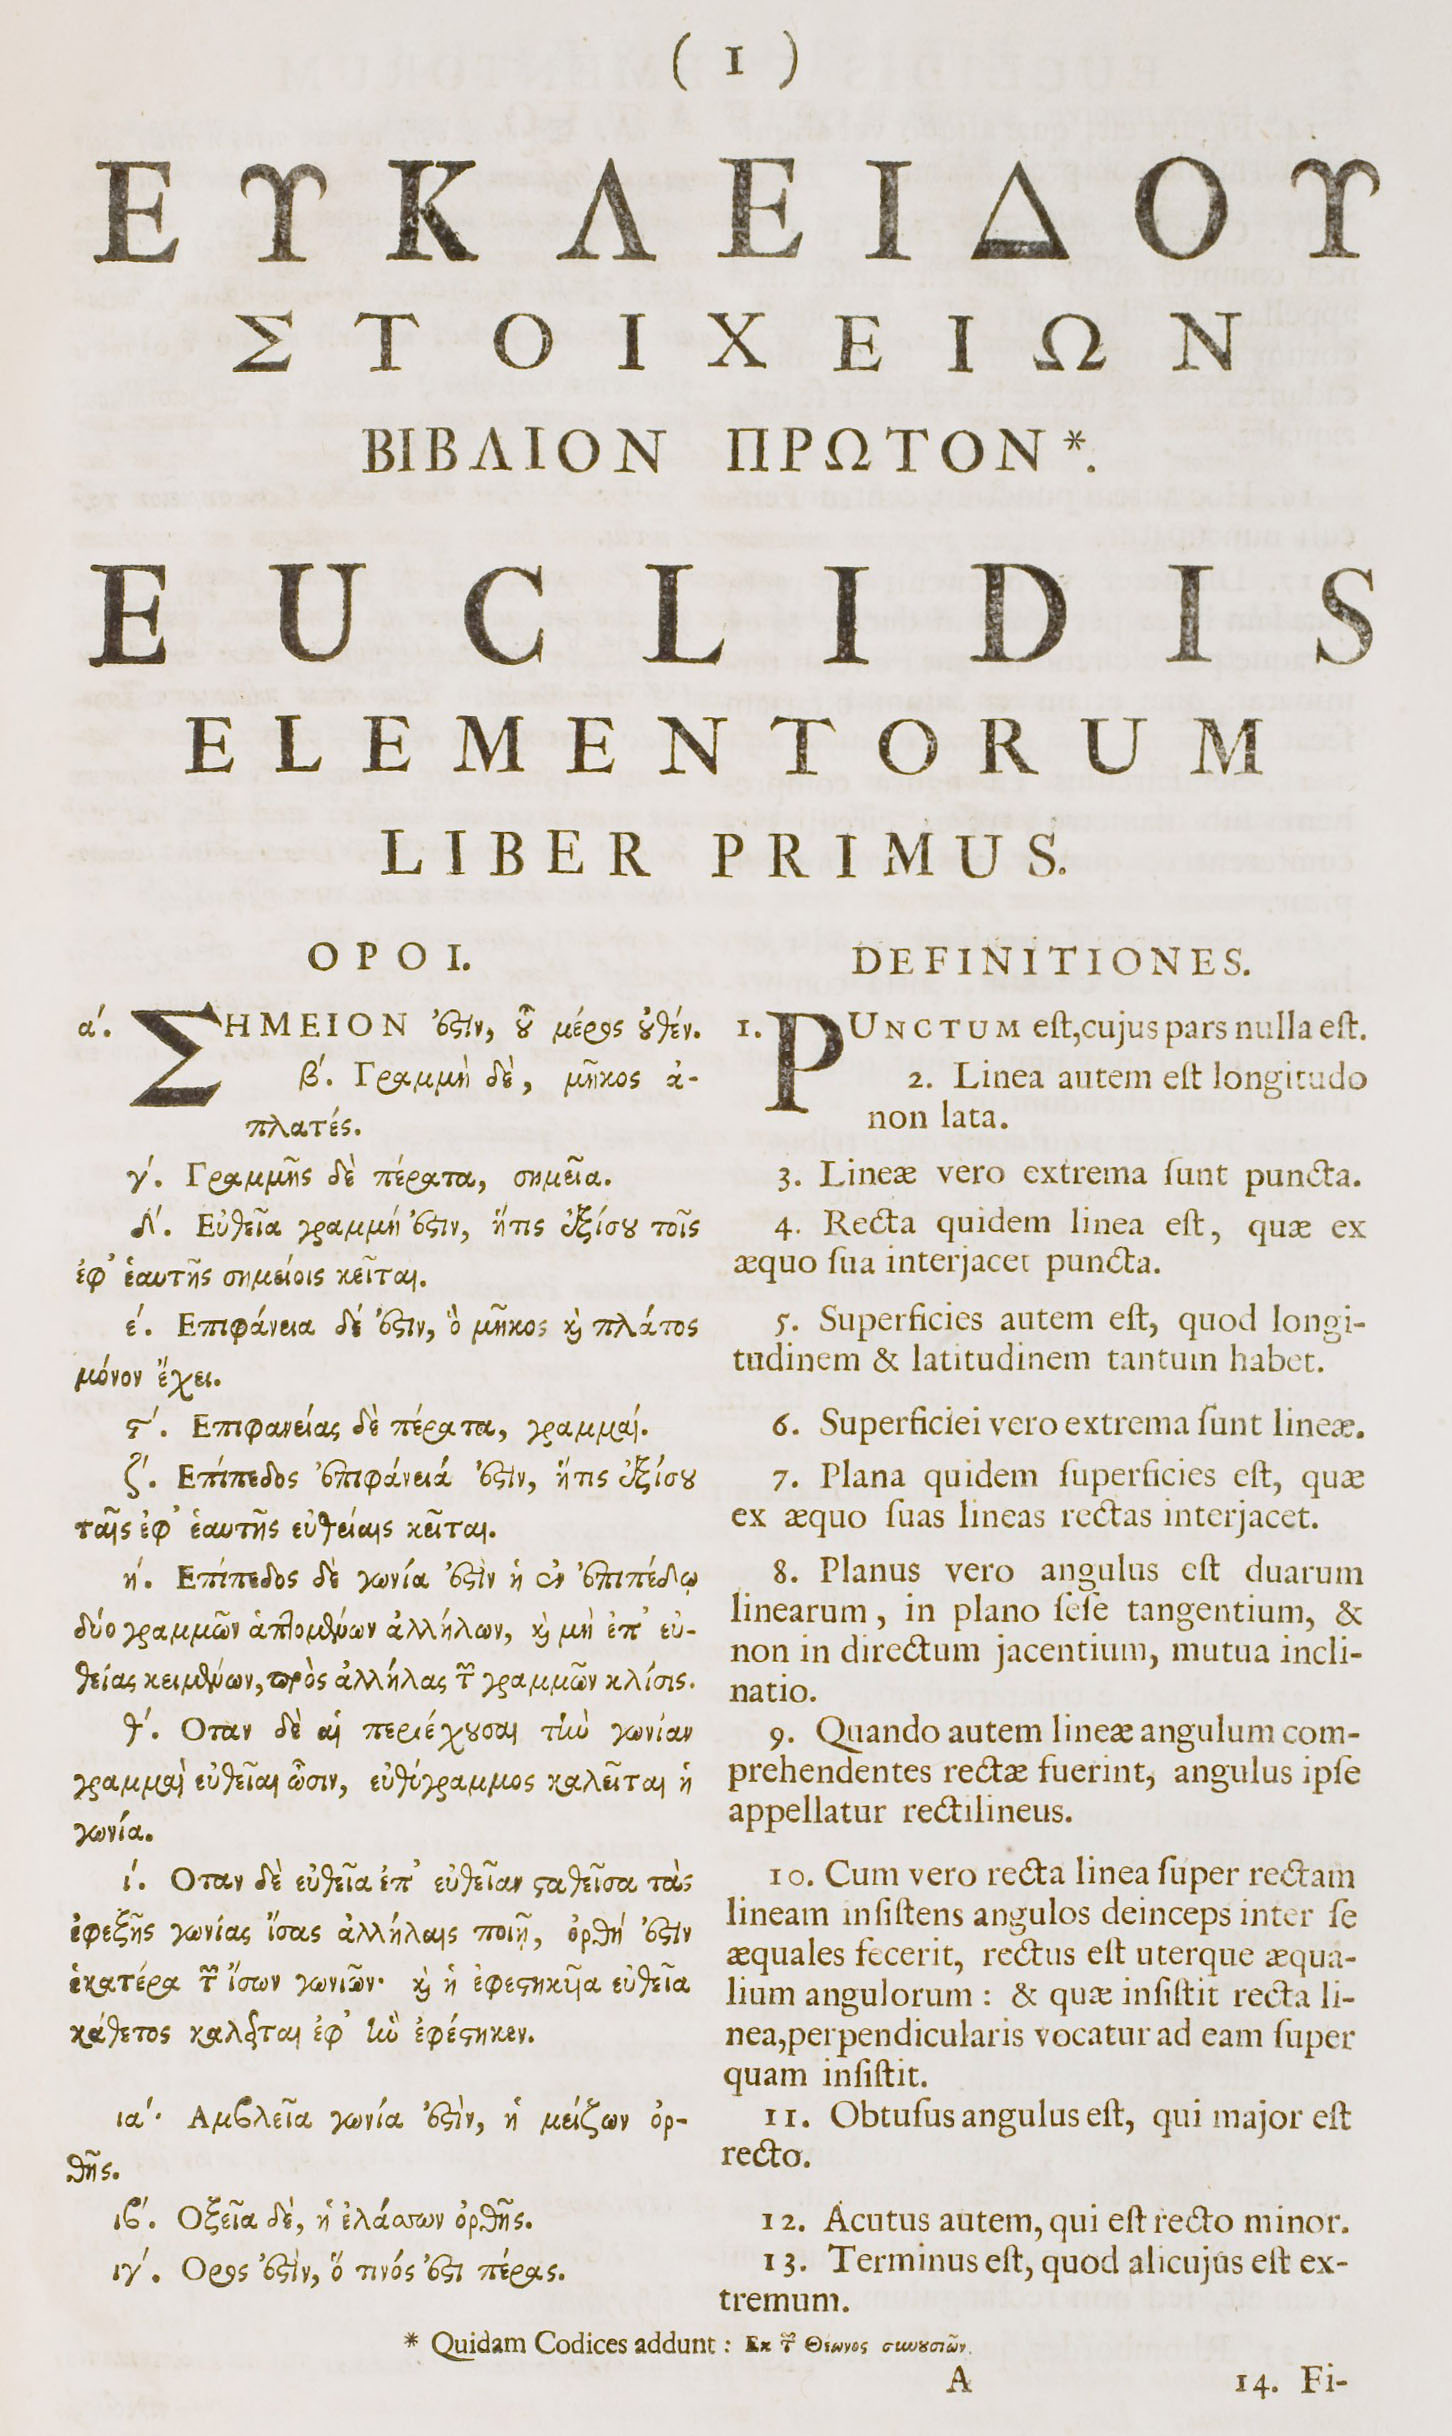
\includegraphics[height=23cm]{euklid_gr_lat_p25_2}
\clearpage

\begin{typeLatin}
\bold{<pb} (1)\bold{>} \\
\bold{<h>}ΕΥΚΛΕΙΔΟΥ \\
ΣΤΟΙΧΕΙΩΝ \\
ΒΙΒΛΙΟΝ ΠΡΩΤΟΝ \bold{<n} *\bold{>}.\bold{</h>} \\
\bold{<h>}EUCLIDIS\\
ELEMENTORUM\\
LIBER PRIMUS.\bold{</h>}\\
\bold{<col 1>}\\
\bold{<h>}ΟΡΟΙ.\bold{</h>}\\
\bold{<p>}α'. ΣΗΜΕΙΟΝ \li{ἐστι}ν, \li{οὗ} μέ\li{ρο}ς \li{οὐ}\li{θέ}ν.\bold{</p>} \\
\bold{<p>}β'. Γ\li{ρα}μ\li{μὴ} \li{δὲ}, \li{μῆ}\li{κο}ς ἀ- \\ 
\li{πλ}ατές.\bold{</p>} \\
\bold{<p>}γ'. Γ\li{ρα}μ\li{μῆ}ς \li{δὲ} \li{πέ}\li{ρα}\li{τα}, \li{ση}μ\li{εῖ}α.\bold{</p>} \\
\bold{<p>}δ'. Εὐ\li{θε}ῖα \li{γρ}αμ\li{μή} \li{ἐστι}ν, ἥ\li{τι}ς \li{ἐξ}ίσ\li{ου} \li{το}ῖς \\ 
ἐφ' ἑ\li{αυ}τῆς \li{ση}μ\li{εί}οις \li{κε}ῖτ\li{αι}.\bold{</p>} \\
\bold{<p>}ε'. Ε\li{πι}φάν\li{ει}α \li{δέ} \li{ἐστι}ν, ὃ \li{μῆ}\li{κο}ς \li{καὶ} \li{πλ}ά\li{το}ς \\ 
\li{μό}νον ἔχ\li{ει}.\bold{</p>} \\
\bold{<p>}ϛ'. Ε\li{πι}φ\li{αν}\li{εί}\li{ας} \li{δὲ} \li{πέ}\li{ρα}\li{τα}, \li{γρ}αμμ\li{αί}.\bold{</p>} \\
\bold{<p>}ζ'. Ε\li{πί}\li{πε}\li{δο}ς \li{ἐπι}φάν\li{ει}ά \li{ἐστι}ν, ἥ\li{τι}ς \li{ἐξ}ίσ\li{ου} \\ 
τ\li{αῖ}ς ἐφ' ἑ\li{αυ}\li{τῆ}ς εὐθ\li{εί}\li{αι}ς κ\li{εῖ}τ\li{αι}.\bold{</p>} \\
\bold{<p>}η'. Ε\li{πί}\li{πε}\li{δο}ς \li{δὲ} \li{γω}νία \li{ἐστὶ}ν ἡ \li{ἐν} \li{ἐπι}\li{πέδ}ῳ \\ 
\li{δύ}ο \li{γρ}αμ\li{μῶ}ν ἁ\li{πτ}ο\li{μέν}ων ἀ\li{λλ}ήλων, \li{καὶ} \li{μὴ} ἐπ' εὐ- \\ 
\li{θε}ί\li{ας} κ\li{ει}\li{μέν}ων, \li{πρ}ὸς ἀ\li{λλ}ήλ\li{ας} \li{τῶν} \li{γρ}αμμῶν κλί\li{σι}ς.\bold{</p>} \\
\bold{<p>}θ'. Ο\li{τα}ν \li{δὲ} \li{αἱ} \li{πε}\li{ρι}έχ\li{ου}\li{σαι} \li{τὴν} \li{γω}νί\li{αν} \\ 
\li{γρ}αμ\li{μαὶ} εὐ\li{θε}ῖ\li{αι} ὦ\li{σι}ν, εὐ\li{θύ}\li{γρ}αμ\li{μο}ς \li{κα}λ\li{εῖ}τ\li{αι} ἡ \\ 
\li{γω}νία.\bold{</p>} \\
\bold{<p>}ι'. Ο\li{τα}ν \li{δὲ} εὐ\li{θε}ῖα ἐπ' εὐ\li{θε}ῖ\li{αν} \li{στα}\li{θε}ῖ\li{σα} \li{τὰ}ς \\ 
ἐφεξῆς \li{γω}νί\li{ας} ἴ\li{σα}ς ἀ\li{λλ}ήλ\li{αι}ς \li{πο}ιῇ, ὀρ\li{θή} \li{ἐστι}ν \\ 
ἑ\li{κα}τέ\li{ρα} \li{τῶν} ἴ\li{σω}ν \li{γω}νιῶν· \li{καὶ} ἡ ἐφε\li{στη}κ\li{υῖ}α εὐ\li{θε}ῖα \\ 
\li{κά}\li{θε}\li{το}ς \li{κα}λ\li{εῖ}τ\li{αι} ἐφ' \li{ἣν} ἐφέ\li{στη}\li{κε}ν.\bold{</p>} \\
\bold{<p>}ια'. Αμβλεῖα \li{γω}νία \li{ἐστὶ}ν, ἡ μ\li{εῖ}ζων ὀρ- \\ 
\li{θῆ}ς.\bold{</p>} \\
\bold{<p>}ιβ'. Οξεῖα \li{δὲ}, ἡ ἐλά\li{σσω}ν ὀρ\li{θῆ}ς.\bold{</p>} \\
\bold{<p>}ιγ'. Ο\li{ρο}ς \li{ἐστὶ}ν, ὅ \li{τι}νός \li{ἐστι} \li{πέ}\li{ρα}ς.\bold{</p>} \\
\bold{</col 1>}\\
\bold{<col 2>}\\
\bold{<h>}DEFINITIONES.\bold{</h>}\\
\bold{<p>}1. PU\bold{<sc>}NCTUM\bold{</sc>} e$t, cujus pars nulla e$t.\bold{</p>}\\
\bold{<p>}2. Linea autem e$t longitudo\\
non lata.\bold{</p>}\\
\bold{<p>}3. Lineæ vero extrema $unt puncta.\bold{</p>}\\
\bold{<p>}4. Recta quidem linea e$t, quæ ex\\
æquo $ua interjacet puncta.\bold{</p>}\\
\bold{<p>}5. Superficies autem e$t, quod longi-\\
tudinem & latitudinem tantum habet.\bold{</p>}\\
\bold{<p>}6. Superficiei vero extrema $unt lineæ.\bold{</p>}\\
\\\untranscribedText \\ \\
\bold{<p>}12. Acutus autem, qui e$t recto minor.\bold{</p>}\\
\bold{<p>}13. Terminus e$t, quod alicujus e$t ex-\\
tremum.\bold{</p>}\\
\bold{</col>} \\
\bold{<fn} *\bold{>}Quidam Codices addunt: Εκ \li{τῶν} Θέωνος σ\li{υν}\li{ου}\li{σι}ῶν.\bold{</fn>} \\
\end{typeLatin}

%\bold{<p>}7. Plana quidem $uperficies e$t, quæ\\
%ex æquo $uas lineas rectas interjacet.\bold{</p>}\\
%\bold{<p>}8. Planus vero angulus e$t duarum\\
%linearum, in plano $e$e tangentium, &\\
%non in directum jacentium, mutua incli-\\
%natio.\bold{</p>}\\
%\bold{<p>}9. Quando autem lineæ angulum com-\\
%prehendentes rectæ fuerint, angulus ip$e\\
%appellatur rectilineus.\bold{</p>}\\
%\bold{<p>}10. Cum vero recta linea $uper rectam\\
%lineam in$i$tens angulos deinceps inter $e\\
%æquales fecerit, rectus e$t uterque æqua-\\
%lium angulorum: & quæ in$i$tit recta li-\\
%nea, perpendicularis vocatur ad eam $uper\\
%quam in$i$tit.\bold{</p>}\\
%\bold{<p>}11. Obtu$us angulus e$t, qui major e$t\\
%recto.\bold{</p>}\\

\begin{note}
%The character §ϛ§, which stands for the number 6, should be typed as U+03DB (Greek small letter stigma).
The character §ϛ§, which occurs only once on this page (in §<p>ϛ'§) and stands for the number 6, is not an end-sigma §ς§, but a stigma. It should be typed as U+03DB (Greek small letter stigma).
%The character §ϛ§, which occurs only once on this page (in §<p>ϛ'§), stands for the number 6. It is not an end-sigma §ς§ and should be typed as U+03DB (Greek small letter stigma).
\end{note}

